% Source for images/process.png, the pipeline diagram in Chapter 2.
% To remake the PNG:
%   cd images && pdflatex process.tex && pdftoppm -png -r 300 -singlefile process.pdf process
\documentclass[border=8pt]{standalone}
\usepackage[T1]{fontenc}
\usepackage[scaled]{helvet}
\renewcommand{\familydefault}{\sfdefault}
\usepackage{tikz}
\usetikzlibrary{arrows.meta, positioning}

\begin{document}
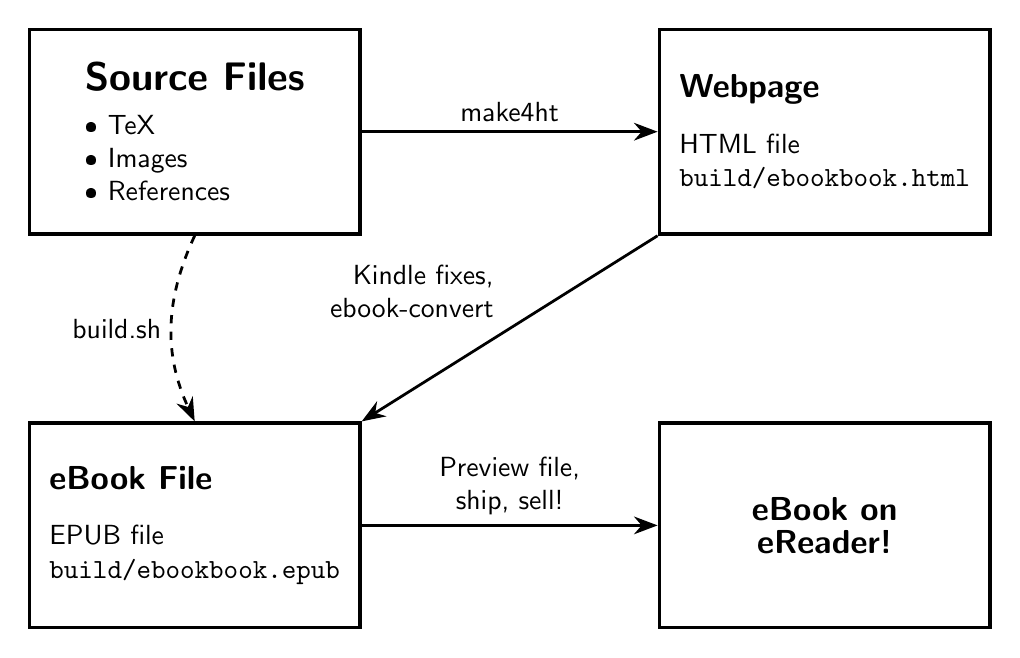
\begin{tikzpicture}[
    box/.style={draw, line width=1.2pt, minimum width=4.2cm, minimum height=2.6cm, align=left},
    arrow/.style={-{Stealth[length=3mm]}, line width=1pt},
  ]
  \node[box] (source) at (0, 0) {\textbf{\Large Source Files}\\[4pt]
    \textbullet\ TeX\\ \textbullet\ Images\\ \textbullet\ References};
  \node[box] (html) at (8, 0) {\textbf{\large Webpage}\\[8pt]
    HTML file\\ \texttt{build/ebookbook.html}};
  \node[box] (epub) at (0, -5) {\textbf{\large eBook File}\\[8pt]
    EPUB file\\ \texttt{build/ebookbook.epub}};
  \node[box, align=center] (reader) at (8, -5) {\textbf{\large eBook on}\\ \textbf{\large eReader!}};

  \draw[arrow] (source) -- node[above, align=center] {make4ht} (html);
  \draw[arrow] (html.south west) -- node[midway, above left=0pt and 2pt, align=right] {Kindle fixes,\\ ebook-convert} (epub.north east);
  \draw[arrow, dashed] (source.south) to[bend right=25] node[left] {build.sh} (epub.north);
  \draw[arrow] (epub) -- node[above, align=center] {Preview file,\\ ship, sell!} (reader);
\end{tikzpicture}
\end{document}
